\documentclass[9pt, addpoints]{exam}
\usepackage[english]{babel}
\usepackage[utf8x]{inputenc}
\usepackage{graphicx,lastpage}
\usepackage{hyperref}
\usepackage{amsmath}
\usepackage{amsthm}
\usepackage{amsfonts}
\usepackage{amssymb}
\usepackage{scrextend}
\usepackage{mathrsfs}
\usepackage{hhline}
\usepackage{booktabs} % book-quality tables
\usepackage{units}    % non-stacked fractions and better unit spacing
\usepackage{multicol} % multiple column layout facilities
\usepackage{lipsum}   % filler text
\usepackage{varwidth} % centering for itemize
\usepackage{listings}
\usepackage[linewidth=1pt]{mdframed}

\renewcommand{\qedsymbol}{$\blacksquare$}

\qformat{\thequestion\dotfill \emph{\totalpoints\ points}}
\pagestyle{headandfoot}
\header{T-409-TSAM}{Assignment 2}{\thepage/\numpages}
\runningheadrule
\firstpagefooter{}{}{}
\runningfooter{}{Page \thepage\ of \numpages}{}

\graphicspath{{.}}
%\printanswers

\title{Assignment 2}

\begin{document}
\noindent
\begin{minipage}[l]{.11\textwidth}%
\noindent
    
\includegraphics[width=\textwidth]{HR}
\end{minipage}%
%\hfill
\begin{minipage}[r]{.6\textwidth}%
\begin{center}
    {\large\bfseries Department of Computer Science \par
    \large Computer Networks \\[2pt]
    \large Due: Monday 23 September (23.59)
    }
\end{center}
\end{minipage}%
\fbox{\begin{minipage}[l]{.4\textwidth}%
\noindent
    {\bfseries Your name:}\\[2pt]
TA Name:    \\
Time Taken: \\
{\footnotesize Estimated Time: {6 hours}}
\end{minipage}}%

\large     
\vspace{2cm}
\begin{center}
    \begin{minipage}{40em}
        \vspace{6pt}
        \begin{center}
            \textbf{This is an individual assignment}
        \end{center}
        \vspace{6pt}

    This assignment can be submitted as a pdf using 
    Canvas.  For those who like to dabble in the dark arts, the latex version 
    is also available, but you may submit in any legible form you wish.
        Marks are awarded for question difficulty. While there is 
        typically a relationship between difficulty and length of answer,
        it may not be a strong one. 
        \\
        \\
        \textbf{Explain your answer or give full derivation
        of results where appropriate. Solitary solutions without explanation
        risk receiving 0 points, even when correct. 
        In particular if there are
        2 points for a short question, 1 of them will be for the explanation.}
        \vspace{12pt}
        \\
        Optional: Please include a rough estimate of how long it took you do the 
        assignment so that we can calibrate the work being assigned for the 
        course. (The estimated time is provided purely as a guideline.)
        \par
        \vspace{12pt}
    \end{minipage}
\end{center}

\vspace{4cm}

\begin{center}
    \gradetable[h]
\end{center}
\newpage

%%% Question 1
\section*{IPv4 Subnetting}
\begin{questions}
 \question
 \begin{parts}
     \part[1] What is the Class A, IP Range 127 used for?
     \vspace{2cm}
     \part[1] What is the Class A, IP Range 224-239 used for?
     \vspace{2cm}
     \part[2] What does a broadcast address instruct the transmitting 
     host to do with the message?
     \vspace{2cm}
     \part[2] What address would you use if you wanted to broadcast to just 
     the local network?
     \vspace{2cm}
     \part[2] What is multicast? 
     \vspace{2cm}
     \part[4] How is it different from broadcast? (Please include a diagram)
 \end{parts}
 \newpage
 \question
     Being able to look at a subnet specification, and list
     the range of the host IPs is a useful, but rather non-obvious
     skill to master in networking. It is also quite often used to screen
     job applicants. The purpose of this question
     is to help you learn it. The following material may be useful:
     
     \url{https://learningnetwork.cisco.com/docs/DOC-10924}
      
    \begin{parts}
     \part[2] What is the network mask for a Class D address?
     \vspace{2cm}

     \part[2] What is the network mask for a Class B address?
     \vspace{2cm}

     \part[2] Using Classless Interdomain Routing(CIDR) notation, how many
     bits are set in the subnet mask of address 10.5.23.132/12
     \vspace{2cm}
     \part[2] How many hosts does this subnet mask provide?
     \vspace{2cm}
 \end{parts}
 \newpage
 \question
 \begin{parts}
     \part[5]{
         In the diagram below, subnet the Class C network of 
         10.5.12.0/24 into 5 subnetworks:
     List the CIDR and IP ranges of each subnet, and show how many hosts are 
     assigned to each subnet.}

       \begin{figure}[ht]
         \centering
         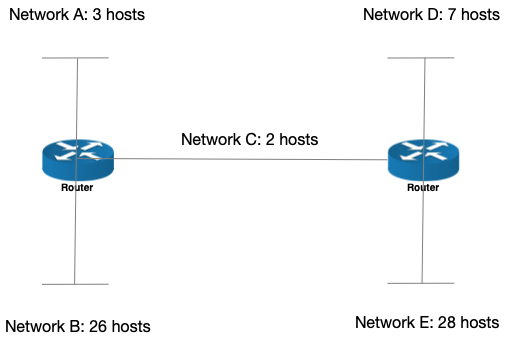
\includegraphics[width=12cm]{subnet}
       \end{figure}
       \vspace{10cm}
     \newpage
     \part[5]{Variable length subnet masks(VLSM) is a feature on some
     equipment that allows different length masks to be used for each subnet, 
     and consequently makes allocating
     address space more efficient. 

     \url{https://www.tutorialspoint.com/ipv4/ipv4_vlsm.htm}
     
     Taking the same network as above,
     develop a subnetting scheme using VLSM with the following 
     requirements:
     \begin{center}
         \begin{tabular}{ll}
             netA & Support 16 hosts \\
             netB & Support 2 hosts \\
             netC & support 5  hosts \\
             netD & support 28 hosts \\
             netE & support 15 hosts \\
          \end{tabular}
     \end{center}
     Once again, list the CIDR and IP ranges for each subnet, and show how
     many host IP addresses are available in each subnet.}
     \vspace{10cm}
 \end{parts}
\newpage
    \section*{Network Address Translation}
    \question
    \begin{parts}
       \begin{figure}[ht]
         \centering
         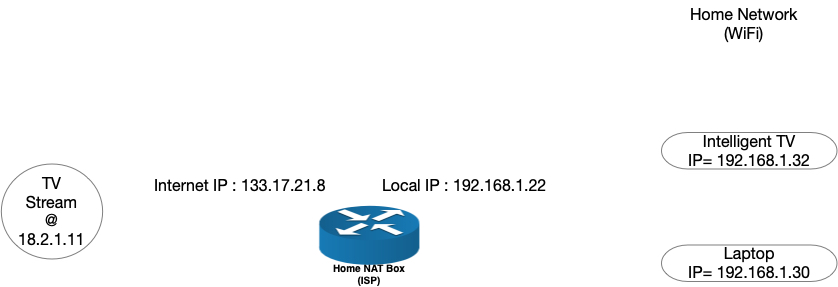
\includegraphics[width=12cm]{nat}
       \end{figure}
         The diagram shows a typical home network setup. 
         The WiFi router has an Internet IP address of 133.17.21.8, 
         and an internal IP address (behind the NAT) of 192.168.1.22

         There is an Intelligent TV (Local IP 192.168.1.32) and a 
         Laptop (192.168.1.30) also on the home network.

    \vspace{1cm}
    \part[4]{Consider that the TV is streaming on its port 8080 from 
        port 54121 on the host for the Internet TV stream at 18.2.1.11 

        Explain for each step of the \textbf{round trip} between the 
        orginating host, and the destination, what address and 
        port are being used. (Hint: fill in a NAT translation table.)}

    \vspace{4cm}
    \part[3] If the Home NAT Box receives a packet from the Internet, 
        addressed to 192.168.1.30, port 8080, what will it do with it?

    \vspace{2cm}
    \part[3] What is the maximum number of connections a NAT box can
        support? Why?
    \end{parts}
\end{questions}
\end{document}
